\documentclass{beamer}
\usepackage[size=custom, width=21, height=27, scale=1.0, orientation=portrait]{beamerposter}
\setbeamertemplate{navigation symbols}{}
\setbeamersize{text margin left=0em,text margin right=0em}

\usepackage{tikz}
\usetikzlibrary{positioning}
\usetikzlibrary{calc}
\usetikzlibrary{arrows,positioning, decorations, decorations.text}

% use Helvetica font
\usepackage{fontspec}
\usefonttheme{serif}
\usepackage{helvet}

%----------------------------------------------------------------------------------------
\begin{document}

\begin{tikzpicture}[remember picture, overlay]

\newcommand{\rowspace}{3.2}
\newcommand{\colspace}{3.5}

\newcommand{\plot}[2]{
  \node[anchor=center, rectangle]
    at (#1) {\includegraphics[height=1.65cm]{#2}};
}

\newcommand{\ylabel}[2]{
  \node at (#1)[anchor=west, text width=2cm, minimum height=1cm] {
  {\footnotesize #2}};
}

\newcommand{\textbox}[2]{
  \node at (#1)[anchor=center] {
  {\footnotesize #2}};
}

\newcommand{\defineRow}[2]{
  \node at ($(top) + (-9.5cm, -#1*\rowspace cm) + (0cm, -1.5cm)$) (#2){};
}

\newcommand{\defineCol}[3]{
  \node at ($(#1) + (#2*\colspace cm, 0cm)$) (#3){};
}


\newcommand{\rowtitle}[1]{
  \node at ($(thisrow) + (0.25cm, 1.5cm)$) [anchor=west, text width=8cm, text height=0.5cm]{
  {\footnotesize #1}};
}

\newcommand{\rowlabel}[1]{
  \node at ($(thisrow) + (0.25cm, 0cm)$)[anchor=west, text width=2cm] {
  \footnotesize {\color{orange!50}  #1}};
}

\newcommand{\firstcol}[4]{
  \defineCol{thisrow}{#1}{thiscol}
  \ylabel{$(thiscol) + (-2.1cm,  0cm)$}{#2}
  \plot{  $(thiscol)$                 }{#3}
  \ylabel{$(thiscol) + (0.7cm,   0cm)$}{=}
  \ylabel{$(thiscol) + (1.1cm,   0cm)$}{#4}
}

\newcommand{\othercol}[4]{
  \defineCol{thisrow}{#1}{thiscol}
  \ylabel{$(thiscol) + (-2.1cm,   0cm)$}{#2}
  \plot{  $(thiscol)$                  }{#3}
  \ylabel{$(thiscol) + (0.85cm,   0cm)$}{#4}
}


\node at ($(current page.south)+ (0cm, 20cm)$) (top){};

\node[rectangle, anchor =south] at ($(top)+ (-5cm, 2cm)$){
  \includegraphics[height= 2cm]{downloads/seedling.png}};
  \textbox{$(top)+ (-5cm, 6.2cm)$}{Seedling}

\node[rectangle, anchor =south] at ($(top)+ (5cm, 0.5cm)$){
  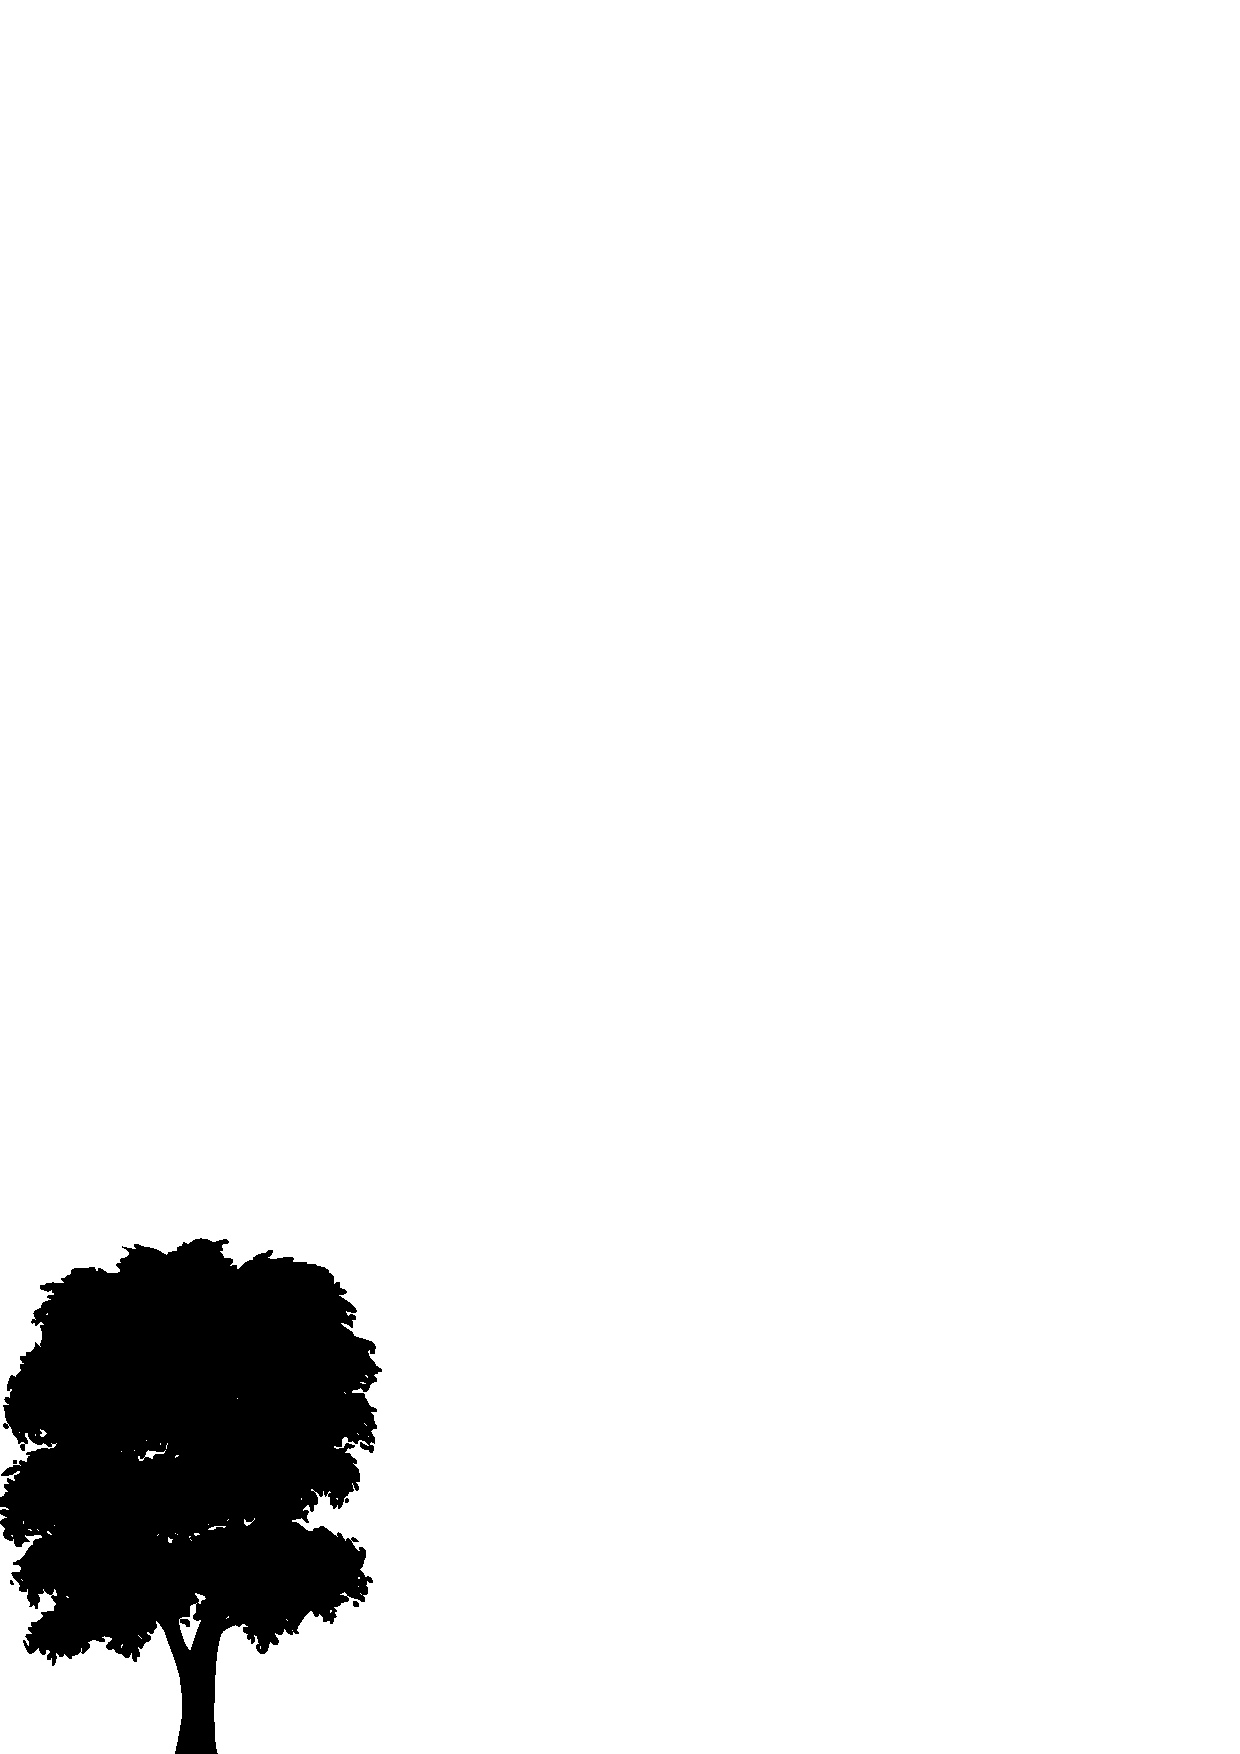
\includegraphics[height= 5cm]{downloads/tree.png}};
  \textbox{$(top)+ (5cm, 6.25cm)$}{Adult}

\defineRow{0}{thisrow}
\rowtitle{Biomass production}
\firstcol{1}{$\frac{\textrm{d}b}{\textrm{d}t}$}{figures/F2_mass_production_net_production}{}
\othercol{2}{$y$}{figures/empty_box}{$\times$}
\othercol{3}{$\Bigg(A$}{figures/F2_mass_production_assimilation}{-}
\othercol{4}{\ $R$}{figures/F2_mass_production_respiration}{$\Bigg)$}
\othercol{5}{$-T$}{figures/F2_mass_production_turnover}{}
\rowlabel{(1)}

\defineRow{1}{thisrow}
\rowtitle{Construction costs}
\firstcol{1}{$\frac{\textrm{d}a_{\textrm{l}}}{\textrm{d}m_{\textrm{t}}}$}{figures/F2_leaf_area_growth_leaf_fraction}{$\Bigg($}
\othercol{2}{$\frac{\textrm{d}m_{\textrm{l}}}{\textrm{d}a_{\textrm{l}}}$}{figures/empty_box}{+}
\othercol{3}{$\frac{\textrm{d}m_{\textrm{ss}}}{\textrm{d}a_{\textrm{l}}}$}{figures/empty_box}{+}
\othercol{4}{$\frac{\textrm{d}m_{\textrm{sb}}}{\textrm{d}a_{\textrm{l}}}$}{figures/empty_box}{+}
\othercol{5}{$\frac{\textrm{d}m_{\textrm{r}}}{\textrm{d}a_{\textrm{l}}}$}{figures/empty_box}{$\Bigg)^{-1}$}
 \rowlabel{(2)}

\defineRow{2}{thisrow}
\rowtitle{Leaf-area growth}
\firstcol{1}{$\frac{\textrm{d}a_{\textrm{l}}}{\textrm{d}t}$}{figures/F2_leaf_area_growth_dleaf_area_dt}{}
\othercol{2}{$\frac{\textrm{d}a_{\textrm{l}}}{\textrm{d}m_{\textrm{t}}}$}{figures/F2_leaf_area_growth_leaf_fraction}{$\times$}
\othercol{3}{$\frac{\textrm{d}m_{\textrm{t}}}{\textrm{d}b}$}{figures/F2_leaf_area_growth_leaf_fraction}{$\times$}
\othercol{4}{$\frac{\textrm{d}b}{\textrm{d}t}$}{figures/F2_leaf_area_growth_net_production}{}
\rowlabel{(3)}

\defineRow{3}{thisrow}
\rowtitle{Height growth}
\firstcol{1}{$\frac{\textrm{d}h}{\textrm{d}t}$}{figures/F2_height_growth_height_growth_rate}{}
\othercol{2}{$\frac{\textrm{d}h}{\textrm{d}a_{\textrm{l}}}$}{figures/F2_height_growth_dheight_dleaf_area}{$\times$}
\othercol{3}{$\frac{\textrm{d}a_{\textrm{l}}}{\textrm{d}t}$}{figures/F2_leaf_area_growth_dleaf_area_dt}{}
\rowlabel{(4)}

\defineRow{4}{thisrow}
\rowtitle{Basal-area growth}
\firstcol{1}{$\frac{\textrm{d}a_{\textrm{st}}}{\textrm{d}t}$}{figures/F2_basal_growth_dbasal_area_dt}{}
\othercol{2}{$\frac{\textrm{d}a_{\textrm{ss}}}{\textrm{d}a_{\textrm{l}}}$}{figures/empty_box}{$\times$}
\othercol{3}{$\frac{\textrm{d}a_{\textrm{l}}}{\textrm{d}t}$}{figures/F2_leaf_area_growth_dleaf_area_dt}{+}
\othercol{4}{$\frac{\textrm{d}a_{\textrm{sh}}}{\textrm{d}t}$}{figures/empty_box}{}
\rowlabel{(5)}

\defineRow{5}{thisrow}
\rowtitle{Diameter growth}
\firstcol{1}{$\frac{\textrm{d}D}{\textrm{d}t}$}{figures/F2_diameter_growth_dbasal_diam_dt}{}
\othercol{2}{$\frac{\sqrt{\pi}}{\sqrt{a_{\textrm{st}}}}$}{figures/empty_box}{$\times$}
\othercol{3}{$\frac{\textrm{d}a_{\textrm{st}}}{\textrm{d}t}$}{figures/F2_basal_growth_dbasal_area_dt}{}
\rowlabel{(6)}

\textbox{$(current page.south)+ (0cm, 0.5cm)$}{Plant height (m)}

\newcommand{\colNum}{0.1}

\defineRow{0}{rowOne}
\defineCol{rowOne}{\colNum}{A}

\defineRow{1}{rowTwo}
\defineCol{rowTwo}{\colNum}{B}

\defineRow{2}{rowThree}
\defineCol{rowThree}{\colNum}{C}

\defineRow{3}{rowFour}
\defineCol{rowFour}{\colNum}{D}

\defineRow{4}{rowFive}
\defineCol{rowFive}{\colNum}{E}

\defineRow{5}{rowSix}
\defineCol{rowSix}{\colNum}{F}

\tikzstyle{s1}=[->,line width=2pt, draw=orange!50]

\draw [s1] (A) to [bend right, looseness=1] (C);
\draw [s1] (B) to [bend right] (C);
\draw [s1] (C) to [bend right, looseness=1] (D);
\draw [s1] (C) to [bend right, looseness=1] (E);
\draw [s1] (E) to [bend right, looseness=1] (F);

\end{tikzpicture}
\end{document}